\chapter{État de l’art}

Actuellement il existe un certain nombre d’applications et de démos dédiés à la plongé et  balades sous-marines. Nous allons vous présenter certaines des ces applications.  

\section{OceanRift}

OceanRift a été créé en 2013 par Llŷr ap Cenydd, conférencier à l’Université de Bangor, au Royaume-Uni, qui est spatialisé dans l’animation procédurale.
L’application vise à immerger l'utilisateur dans un monde sous-mari. L'idée est de combiner différentes techniques pour simuler une expérience sous-marin vif en réalité virtuelle. Cela comprend à expérimenter avec différents sons, des animaux, la vie végétale, des effets des courants océaniques, les systèmes de particules (poussière, bulles etc.).


\begin{figure}[!ht]
	\center	
	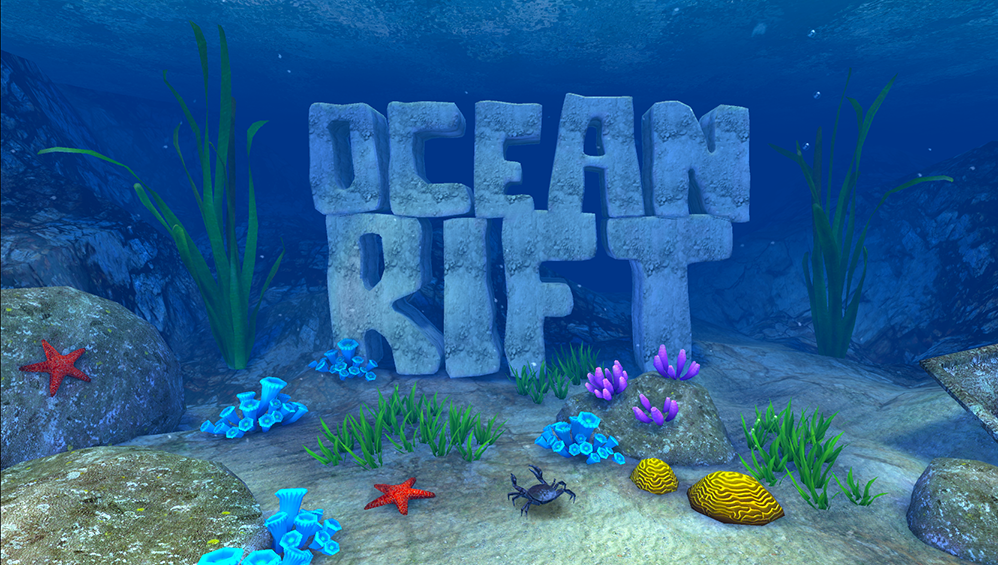
\includegraphics[scale=0.4]{image/OceanRift.png}
	\caption{Ocean-Rift}
\end{figure}

Information \cite{2} \cite{3}:
\begin{table}[h]
	\center	
\begin{tabular}{|l|l|}
\hline
 Prix:  & Gratuit \\ \hline
 Titre PC  &  Ocean Rift 3D Oculus Rift \\ \hline
 Driver nécessaire  &  3D Native Oculus Rift \\ \hline
 Catégorie  &  Démo techno \\ \hline
 Support RV  &  Oculus Rift DK1, Oculus Rift DK2, Gamepad\\ \hline
 Matériel  &  3D Oculus Rift Dev Kit \\ \hline
 Configuration  &  PC avec Carte vidéo 3D Geforce GTX 670 / 8 Go RAM  \\ \hline
\end{tabular}
\end{table}

\newpage

\section{World of Diving}

World of Diving est un jeu de plongée multijoueur, développé par la société Vertigo Games en 2014, qui permet d’exploiter le monde sous-marin. Le bute du jeu est de suivre et de photographier la faune marine, faire face à des dysfonctionnements technique, survivre à des scénarios catastrophes, faire une chasse au trésor, etc. Le jeu donne à l’utilisateur la possibilité de personnaliser son personnage, de faire un équipe et jouer avec d’autre personnes.

\begin{figure}[!ht]
	\center	
	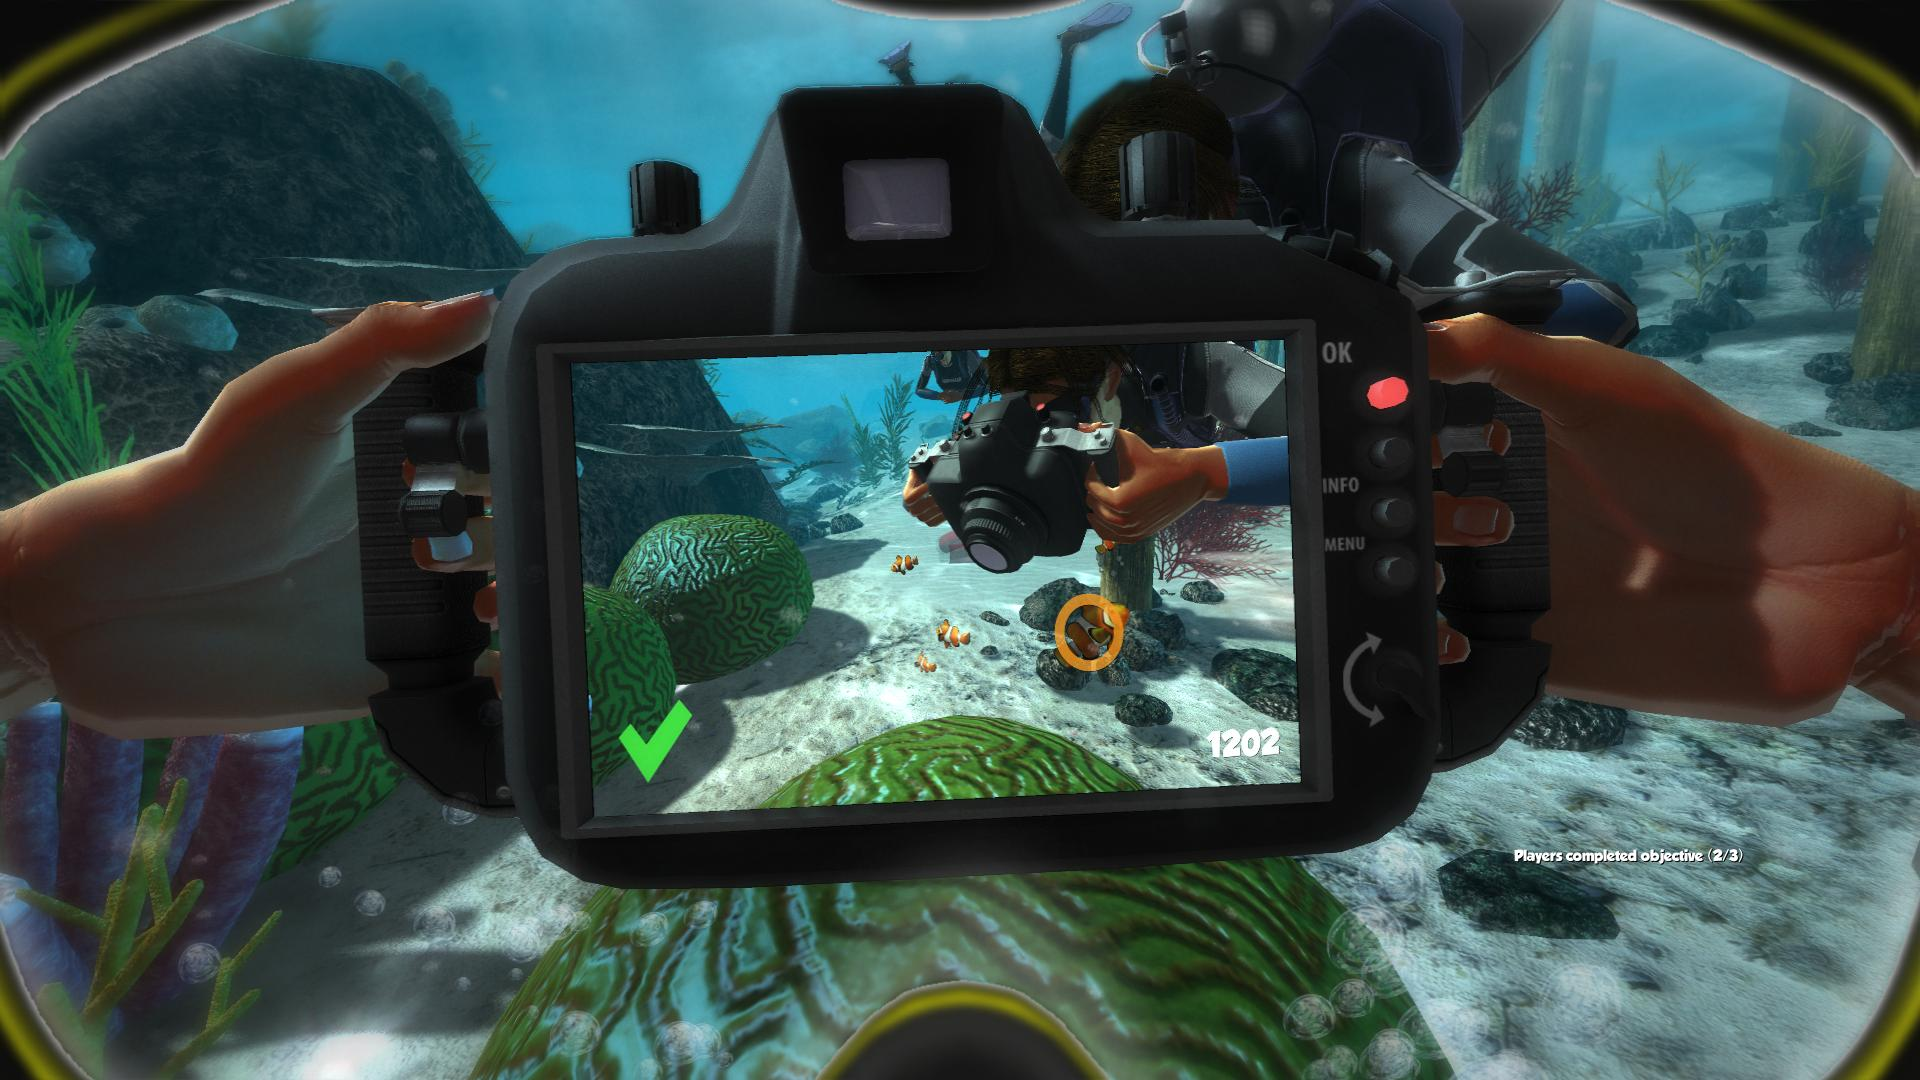
\includegraphics[scale=0.2]{image/worldOf.jpg}
	\caption{World Of Diving}
\end{figure}

Information \cite{4}:
\begin{table}[h]
	\center	
\begin{tabular}{|l|l|}
\hline
 Prix:  & 20 \textdollar \\ \hline
Genre  &  Massively Multiplayer, Casual, Simulation \\ \hline
 Joueurs  &  Single-player, Multi-player, Cross-Platform Multiplayer \\ \hline
 Plateformes  &  Windows, OSX, Linux \\ \hline
 Support RV  &  Oculus Rift \\ \hline
 Developpeur  &  Vertigo Games \\ \hline
 Distribution  &  Digital distribution  \\ \hline
\end{tabular}
\end{table}

\section{UnderCurrent}

Undercurrent est un jeu d'aventure sous-marin pour l'Oculus Rift dans lequel le joueur contrôle un véhicule souterrain appelé The Marv. Le but est de remplir les réserves d'oxygène, résoudre des énigmes, échapper à des monstres souterrains, etc.

\begin{figure}[!ht]
	\center	
	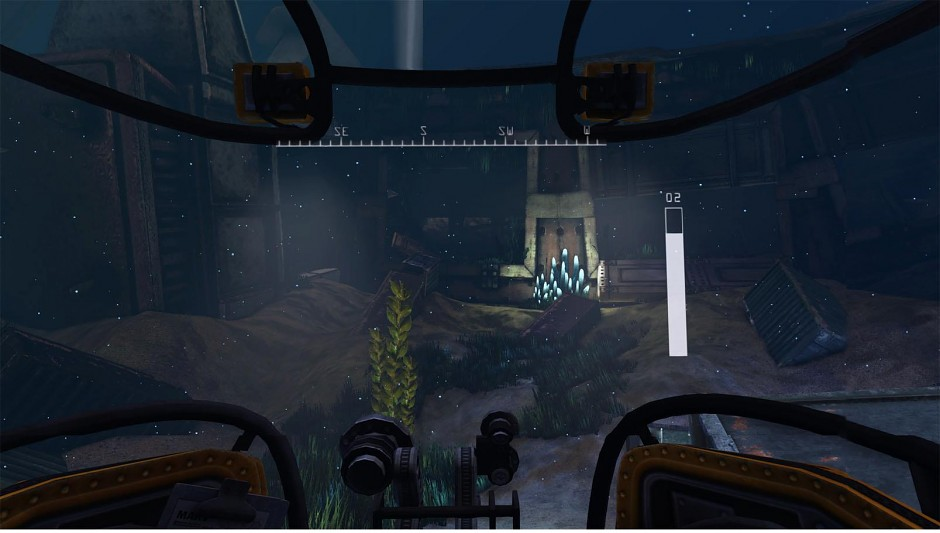
\includegraphics[scale=0.4]{image/under.jpg}
	\caption{UnderCurrent}
\end{figure}


Information \cite{5}:
\begin{table}[h]
	\center	
\begin{tabular}{|l|l|}
\hline
 Prix:  & Gratuit \\ \hline
Genre  &  Aventure \\ \hline
 Plateformes  &  Windows \\ \hline
 Support RV  &  Oculus Rift \\ \hline
 Moteur  &  Unreal Development Kit \\ \hline
 Distribution  &  Hammerhead Studios  \\ \hline
\end{tabular}
\end{table}

\newpage

\section{Synthèse}

Actuellement il n'existe aucune attraction qui pourrait être comparée à notre projet par le niveau d'immersion et la richesse des sensations. Les seuls produits existants permettent d’assurer seulement le coté visuel de l’expérience. Même si certaines applications sont très réalistes, le seul fait de voir le fond marin ne compense pas l’absence du ressentit de l'eau. 

Notre projet est donc une nouvelle expérience qui permettra d'avoir un retour visuel, comme il existe acutellement, mais également un retour sensoriel de part l'immersion totale de l'utilisateur dans l'eau.
